%======================================================================
% End Matter (part of the Letter, NOT the Supplementary Material).
% \input by the main file Draft3.tex.
%======================================================================
% The combined architecture/orchestration figure is pinned as a full-width
% block so it appears at the start of the End Matter; REVTeX figure* floats
% otherwise tend to move it onto a later or isolated float page.
% fig_architecture_combined.tex  -  Architecture (left, 7) + orchestration
% patterns (right, 3), combined into a single full-width (figure*) row so
% both fit one figure in the end matter, separated by a vertical rule
% (a tabular column rule spans the full row height automatically).  The
% architecture panel is the original three-tier layout from
% fig_architecture.tex (human on top, orchestrator, five agents), just
% resized to share the row with the orchestration-pattern panel.
% Requires:  \usepackage{tikz}
%            \usetikzlibrary{arrows.meta, positioning, calc, fit, backgrounds}

% Pinned page-wide block instead of a figure* float: placed at the very top
% of the End Matter's first page (see note in endmatter.tex). The caption
% still numbers as a figure via \def\@captype{figure}.
\onecolumngrid
\begin{center}
% 6pt gutters (8pt overflowed \textwidth by 1.1pt with the 0.63+0.34 panels)
\begin{tabular}{@{}c@{\hspace{12pt}}c@{}}
\resizebox{0.63\linewidth}{!}{%
\begin{tikzpicture}[
    >={Stealth[length=3.2pt]},
    every node/.style ={font=\footnotesize},
    box/.style    ={draw, rounded corners=1.5pt, inner sep=2pt,
                    align=center, font=\scriptsize, minimum height=0.50cm},
    agent/.style  ={box, agentbox, minimum width=1.95cm},
    human/.style  ={box, humanbox},
    sandbox/.style={resourcebox, rounded corners=3pt, inner sep=10pt},
    chip/.style   ={font=\small\itshape, fill=white, inner sep=1.5pt,
                    rounded corners=1pt, draw=black!40, dashed},
    legsw/.style  ={draw, minimum size=0.26cm, inner sep=0pt,
                    rounded corners=0.5pt},
    flow/.style   ={->, semithick, draw=black!80}
  ]

  %% --- Top: human supervisor (grey, not an agent) ---------------------
  \node[human, font=\footnotesize\itshape, minimum width=2.2cm] (human) at (0,2.55)
      {Human \scriptsize(mathematical oversight)};

  %% --- Orchestrator (lead AI agent) -----------------------------------
  \node[agent, minimum width=3.6cm] (orch) at (0,1.40)
      {\texttt{leanOrchestrator}\\\scriptsize planning, delegation, integration};

  %% --- Five front-line AI agents --------------------------------------
  \node[agent] (scout) at (-5.4,0)
      {\texttt{leanSearch}\\\scriptsize Mathlib search};
  \node[agent] (proof) at (-2.7,0)
      {\texttt{lean}\\\scriptsize proofs, sorry closure};
  \node[agent] (clean) at (0,0)
      {\texttt{leanSimplifier}\\\scriptsize lint, simplify};
  \node[agent] (bp) at (2.7,0)
      {\texttt{leanBlueprint}\\\scriptsize \LaTeX{} sync};
  \node[agent] (audit) at (5.4,0)
      {reviewer\\\scriptsize hypothesis audit};

  %% --- Shared sandbox (drawn behind so it does not overpaint nodes);
  %%     a phantom coordinate below the agents gives the chip extra
  %%     room without pushing the top edge into the human box ---------
  \coordinate (padbottom) at ($(scout.south)+(0,-16pt)$);
  \begin{pgfonlayer}{background}
    \node[sandbox, fit=(orch)(scout)(audit)(padbottom)] (sandbox) {};
  \end{pgfonlayer}
  \node[chip, anchor=south]
      at ([yshift=-5pt]sandbox.south)
      {shared by every agent: persistent memory $\cdot$ Lean 4 server (\texttt{diagnostics}, \texttt{inspect}, \texttt{loogle})};

  %% --- Legend: role is encoded by box fill/outline (sits in the empty
  %%     upper-right of the sandbox interior) ----------------------------
  \node[legsw, agentbox] (lg1) at (4.0,1.6) {};
  \node[anchor=west, font=\scriptsize] (lg1t) at (lg1.east) {AI agent};
  \node[legsw, humanbox,
        below=3pt of lg1.south, anchor=north] (lg2) {};
  \node[anchor=west, font=\scriptsize] (lg2t) at (lg2.east) {human supervisor};
  \node[legsw, resourcebox,
        below=3pt of lg2.south, anchor=north] (lg3) {};
  \node[anchor=west, font=\scriptsize] (lg3t) at (lg3.east) {shared resource};
  \begin{pgfonlayer}{background}
    \node[draw=black!20, rounded corners=2pt, fill=white, inner sep=4pt,
          fit=(lg1)(lg1t)(lg2t)(lg3)(lg3t)] {};
  \end{pgfonlayer}

  %% --- Control edges (solid): human -> orch -> agents -----------------
  \draw[flow] (human) -- (orch);
  \foreach \n in {scout,proof,clean,bp,audit}
      \draw[flow] (orch.south) -- (\n.north);
\end{tikzpicture}%
}
&
\resizebox{0.34\linewidth}{!}{%
\begin{tikzpicture}[
        >={Stealth[length=3.2pt]},
        every node/.style={font=\footnotesize},
        box/.style   ={draw, rounded corners=1pt, minimum width=1.05cm,
                minimum height=0.42cm, inner sep=1.5pt, font=\footnotesize},
        agent/.style ={box, agentbox},
        % white fill: a grey fill here read as the legend's "human" encoding
        op/.style    ={box, draw=black!70, fill=white, font=\footnotesize\itshape},
        flow/.style  ={->, semithick, draw=black!75},
        caplbl/.style={font=\footnotesize\bfseries},
        sub/.style   ={font=\footnotesize\itshape, text=black!65},
        edgelbl/.style={font=\scriptsize, inner sep=1pt, fill=white}
    ]

    %% --- Panel A: Parallel dispatch (left half) ------------------------
    \begin{scope}[local bounding box=panelA]
        \node[agent] (orchA) at (0,1.25) {orchestrator};
        % 1.22cm pitch: at the old 1.10 the three boxes nearly abutted after
        % the 0.34\linewidth resize and read as one subdivided bar
        \node[agent] (a1) at (-1.22,0.20) {$T_1$};
        \node[agent] (a2) at ( 0.00,0.20) {$T_2$};
        \node[agent] (a3) at ( 1.22,0.20) {$T_3$};
        \node[op] (mg) at ( 0.00,-0.85) {merge};
        \foreach \n in {a1,a2,a3} \draw[flow] (orchA) -- (\n);
        \foreach \n in {a1,a2,a3} \draw[flow] (\n) -- (mg);
        \node[caplbl] at (0,-1.55) {(a) Parallel dispatch};
        \node[sub]    at (0,-1.92) {disjoint scopes};
    \end{scope}

    %% --- Panel B: Scout-then-prove (top right); named as in the End
    %%     Matter text, which cites the panels individually ---------------
    \begin{scope}[shift={(3.95,0.95)}, local bounding box=panelB]
        \node[caplbl] at (0,0.70) {(b) Scout--then--prove};
        \node[agent] (sc) at (-1.05,0) {scout};
        \node[agent] (im) at ( 1.05,0) {prover};
        % unfilled label lifted clear of the box tops: a white-filled 'memo'
        % here erased the corners of the scout/implementer outlines
        \draw[flow] (sc) -- node[edgelbl, fill=none, above=3pt]{memo} (im);
        \node[sub] at (-1.05,-0.40) {cheap};
        \node[sub] at ( 1.05,-0.40) {expensive};
    \end{scope}

    %% --- Panel C: Review-repair loop (bottom right) --------------------
    \begin{scope}[shift={(3.95,-1.05)}, local bounding box=panelC]
        \node[caplbl] at (0,0.75) {(c) Review--repair loop};
        \node[agent] (aud) at (-0.95,0) {reviewer};
        \node[agent] (fix) at ( 0.95,0) {fixer};
        \draw[flow] (aud) to[bend left=28]
        node[edgelbl, above]{issues} (fix);
        \draw[flow] (fix) to[bend left=28]
        node[edgelbl, below]{patch} (aud);
        \draw[flow, dashed] (aud.south) -- ++(0,-0.55)
        node[edgelbl, below, fill=none]{accept};
        \node[sub] at (0.55,-0.85) {$\le 5$ iterations};
    \end{scope}

\end{tikzpicture}%
}
\end{tabular}
\end{center}
\begingroup
\makeatletter\def\@captype{figure}\makeatother
\caption{%
    System architecture and orchestration patterns.
    \emph{Left}: a human
    supervisor sets mathematical intent; the orchestrator dispatches to
    four specialized interactive agents: a library scout (\texttt{leanSearch}), a
    proof writer (\texttt{lean}), a simplifier (\texttt{leanSimplifier}), and
    a blueprint synchronizer (\texttt{leanBlueprint}), together with an
    automated reviewer that also runs on each change proposed to the shared
    repository. All interactive agents
    (including the orchestrator) share a persistent memory and the
    Lean~4 server's \texttt{diagnostics}, \texttt{inspect}, and
    \texttt{loogle} tools (Supplementary Material~\cite{Supp}), drawn as a single
    dashed region rather than one connection per agent per service.
    \emph{Right}: the three recurring orchestration patterns.
    \textbf{(a)} The orchestrator dispatches independent subtasks
    $T_1,\dots,T_n$ to workers on disjoint scopes and merges their
    outputs. \textbf{(b)} A cheap scout surveys the library and emits a
    design memo which a stronger prover consumes, so the expensive
    proof agent is invoked only after a feasible route is
    identified. \textbf{(c)} A
    reviewer flags issues and a fixer applies patches; the loop
    terminates when the reviewer accepts (dashed) or after a cap of
    five iterations.%
}\label{fig:architecture}\label{fig:orchestration}
\endgroup
\vspace{0.5\baselineskip}
\twocolumngrid


\section*{Method: Multi-agent autoformalization}
%======================================================================


The formalization was produced by a team of specialized language-model agents coordinated through the shared blueprint and a persistent memory; here an agent is a language-model program that edits files and responds to Lean's type-checking feedback until its task is complete. This End Matter describes the agent roles, the blueprint and memory that coordinate them, and the software built to run them; the Supplementary Material~\cite{Supp} expands each part, reproduces the agent prompts, and reports the full cost analysis.

\prlsection{Multi-agent architecture and implementation}
The proof development is organized around six specialized agent roles: proof writer, library scout, simplifier, blueprint synchronizer, orchestrator, and reviewer; the last runs automatically on each change proposed to the shared repository. The other five agents work in interactive sessions and share the blueprint and a persistent memory of notes on what has been tried, what worked, and what failed; \cref{fig:architecture} shows the resulting system architecture. Each of these five agents interacts with Lean~4 through file editing and real-time type-checking feedback, the same interface a human developer uses in editors such as VS Code~\cite{MicrosoftCorporation2024Visual}. Proof writing is assigned to the most capable, most expensive language models, since proof errors propagate downstream; scouting, cleanup, and auditing use less expensive models, since failed attempts are cheap to retry; orchestration uses either class of model, according to the complexity of the task. The resulting usage by role is shown in \cref{fig:role_model_main}, and \cref{fig:model_gantt_main} shows when each model was in use over the project; the full cost analysis appears in the Supplementary Material~\cite{Supp}.

These six roles were not fixed from the start: whenever a recurring bottleneck appeared, often reported by the agents themselves, the supervisor introduced a new role for the missing function, and the full set was in place within the first six weeks of the project.

The agents interact through a small set of recurring coordination patterns: parallel dispatch, shown in panel~(a) of \cref{fig:orchestration}, where the orchestrator sends out many independent tasks; scout-then-prove, shown in panel~(b) of \cref{fig:orchestration}, where a scout runs an inexpensive library search before the prover attempts a costly proof; and review-repair cycles, shown in panel~(c) of \cref{fig:orchestration}, where a reviewer-fixer pair cycles through review and repair. Scout-then-prove was reused most often: a fast, inexpensive agent first identifies the relevant existing results in Mathlib, and a more capable agent then uses them to construct the proof. The remaining agents audit and reorganize in review-repair cycles: the blueprint synchronizer keeps the blueprint and the Lean code in step, the simplifier compresses long proofs, and the reviewer cross-checks claims against the primary literature.

The system we build and use is not an off-the-shelf coding assistant like Claude Code or Codex.
The system is built from the language-model interfaces (API calls) as a software that runs the agents, TeXRA~\cite{TeXRA}; the Lean-specific roles, tools, and prompts are additions built for this project.
The agent prompts and role definitions are released with TNLean~\cite{TNLean}; TeXRA itself is available separately, and the system prompts of the interactive roles are reproduced in the Supplementary Material~\cite{Supp}.

\begin{figure}[!htb]
    \centering
    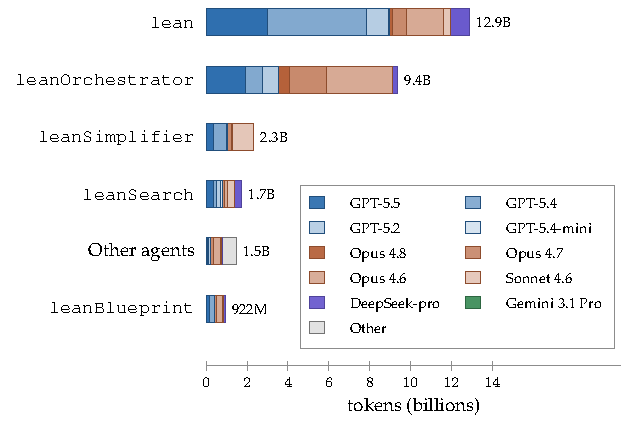
\includegraphics[width=\linewidth]{figures/costs/fig_role_model_tokens.pdf}
    \caption{Token usage by agent role, each bar broken down by the
        language models that role used. Proof writing and orchestration
        dominate, consistent with assigning the most capable models to the
        tasks where an error is most expensive.}\label{fig:role_model_main}
\end{figure}

\begin{figure}[!htb]
    \centering
    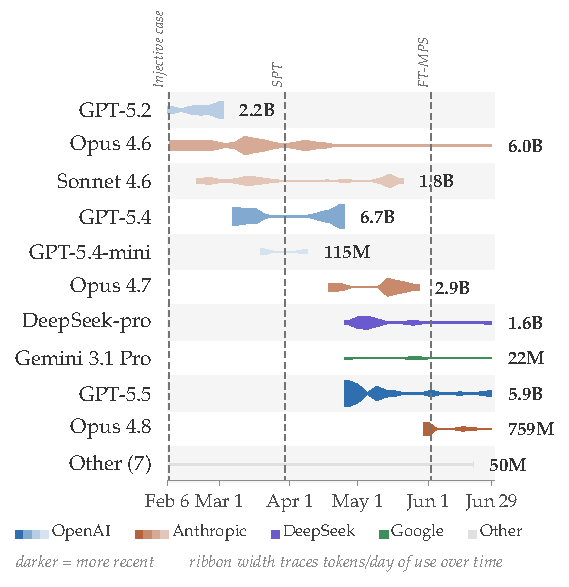
\includegraphics[width=\linewidth]{figures/costs/fig_model_gantt_tokens.pdf}
    \caption{Model usage over the project. Newer model releases
        progressively replaced older ones within each provider family, and the
        token usage concentrated on the most capable models available at each
        time. Each model's period of use is shown as a ribbon, sorted by first
        use: one color family per provider, shade distinguishing models within a
        family, and ribbon width tracing the daily token usage on one scale
        shared across every model; the number at the end of each ribbon is that
        model's total. The dashed vertical lines mark the dates the injective
        case of FT-MPS, the SPT cohomological invariant, and the FT-MPS proof
        chains reported in this work became fully verified.}\label{fig:model_gantt_main}
\end{figure}

\prlsection{Blueprint, memory, and human oversight}
Two shared elements support this architecture: the blueprint and the persistent memory. Every definition, lemma, and theorem in the blueprint carries a proof sketch, a proof status, and its logical dependencies, and is linked to the Lean declarations that formalize it~\cite{Massot2021Leanblueprint}. A theorem stated across several sources in different notations is written once in the blueprint and then proved in Lean, so the blueprint sits between the primary literature and the Lean code (\cref{fig:alignment}). The blueprint is publicly available~\cite{TNLeanBlueprint}, and the Supplementary Material~\cite{Supp} reproduces the portion of its dependency graph around the fundamental theorem at print scale. The persistent memory separately records scouting results, proof strategies, counterexamples, and technique notes across sessions (the bounded working periods after which an agent's conversation is set aside and no longer read by later agents); without it, each dead end would be re-investigated from scratch.

The blueprint is also where the project separates \textit{tactical} from \textit{strategic} decisions. Tactical decisions belong to the agents: which Mathlib lemmas to invoke, when to abandon a failed approach, how to decompose a long argument into intermediate lemmas, and what definitions to try for MPS tensors and transfer operators, down to how the \nFilesfull{} source files of the full library are organized. Strategic decisions remain with the human supervisor: whether the formal statement is the theorem intended by the primary literature, and whether its hypotheses are correct. The supervisor acts through blueprint review and by steering the orchestrator (assigning stronger or more economical models to each task, redirecting the orchestrator away from unproductive routes), never by writing Lean code or choosing proof tactics; the supervision effort therefore does not grow with the length of individual proofs, since Lean already checks each proof. The supervisor reviewed the blueprint in \nReviewRounds{} rounds, each assisted by separate review agents that cross-checked chapters against the primary literature~\cite{Perez-Garcia2007Matrix,Cirac2017Matrixa,Cirac2021Matrix,Sanz2010Quantum}; each round surfaced 10--30 issues, chiefly missing hypotheses, mismatched definitions, and overly general claims, of which the doubly-stochastic gauge and the asymptotic reformulation traced in the main text are representative. This division of labor proved effective: most tactical decisions survived blueprint review, and where they did not, the review traced the error to a definition or an unintended hypothesis, which the agents then corrected.

As anticipated in the Introduction, no language-model context window can hold the source literature, the growing blueprint, and the expanding formal library at once; the work is therefore split into the many bounded sessions coordinated above. Within a session, too, the orchestrator's own conversation grows until it must be condensed: older exchanges are replaced by summaries while the list of running agents and open tasks is retained, so durable knowledge resides in the persistent memory rather than in any one conversation. This memory is what lets a fixed context window, and a fixed amount of supervisor effort, span a project far larger than either could otherwise hold.
